\documentclass[12pt,prb,aps,epsf]{report}
\usepackage[utf8]{inputenc}
\usepackage{amsmath}
\usepackage{amsfonts}
\usepackage{amssymb}
\usepackage{graphicx} 
\usepackage{latexsym} 
\usepackage[toc,page]{appendix}
\usepackage{listings}
\usepackage{xcolor}
\usepackage{soul}
\usepackage[T1]{fontenc}
\usepackage{amsthm}
\usepackage{mathtools}
\usepackage{setspace}
\usepackage{array,multirow,makecell}
\usepackage{geometry}
\usepackage{textcomp}
\usepackage{float}
%\usepackage{siunitx}
\usepackage{cancel}
%\usepackage{tikz}
%\usetikzlibrary{calc, shapes, backgrounds, arrows, decorations.pathmorphing, positioning, fit, petri, tikzmark}
\usepackage{here}
\usepackage{titlesec}
%\usepackage{bm}
\usepackage{bbold}

\geometry{hmargin=2cm,vmargin=2cm}

\begin{document}
	
	\title{MP 09 Diffraction d'ondes lumineuses}
	\author{Matthieu}
	
	\maketitle
	
	\tableofcontents
	
	\pagebreak
	
	
\section{Diffraction par une fente rectangulaire}
\begin{figure}[h]
	\centerline{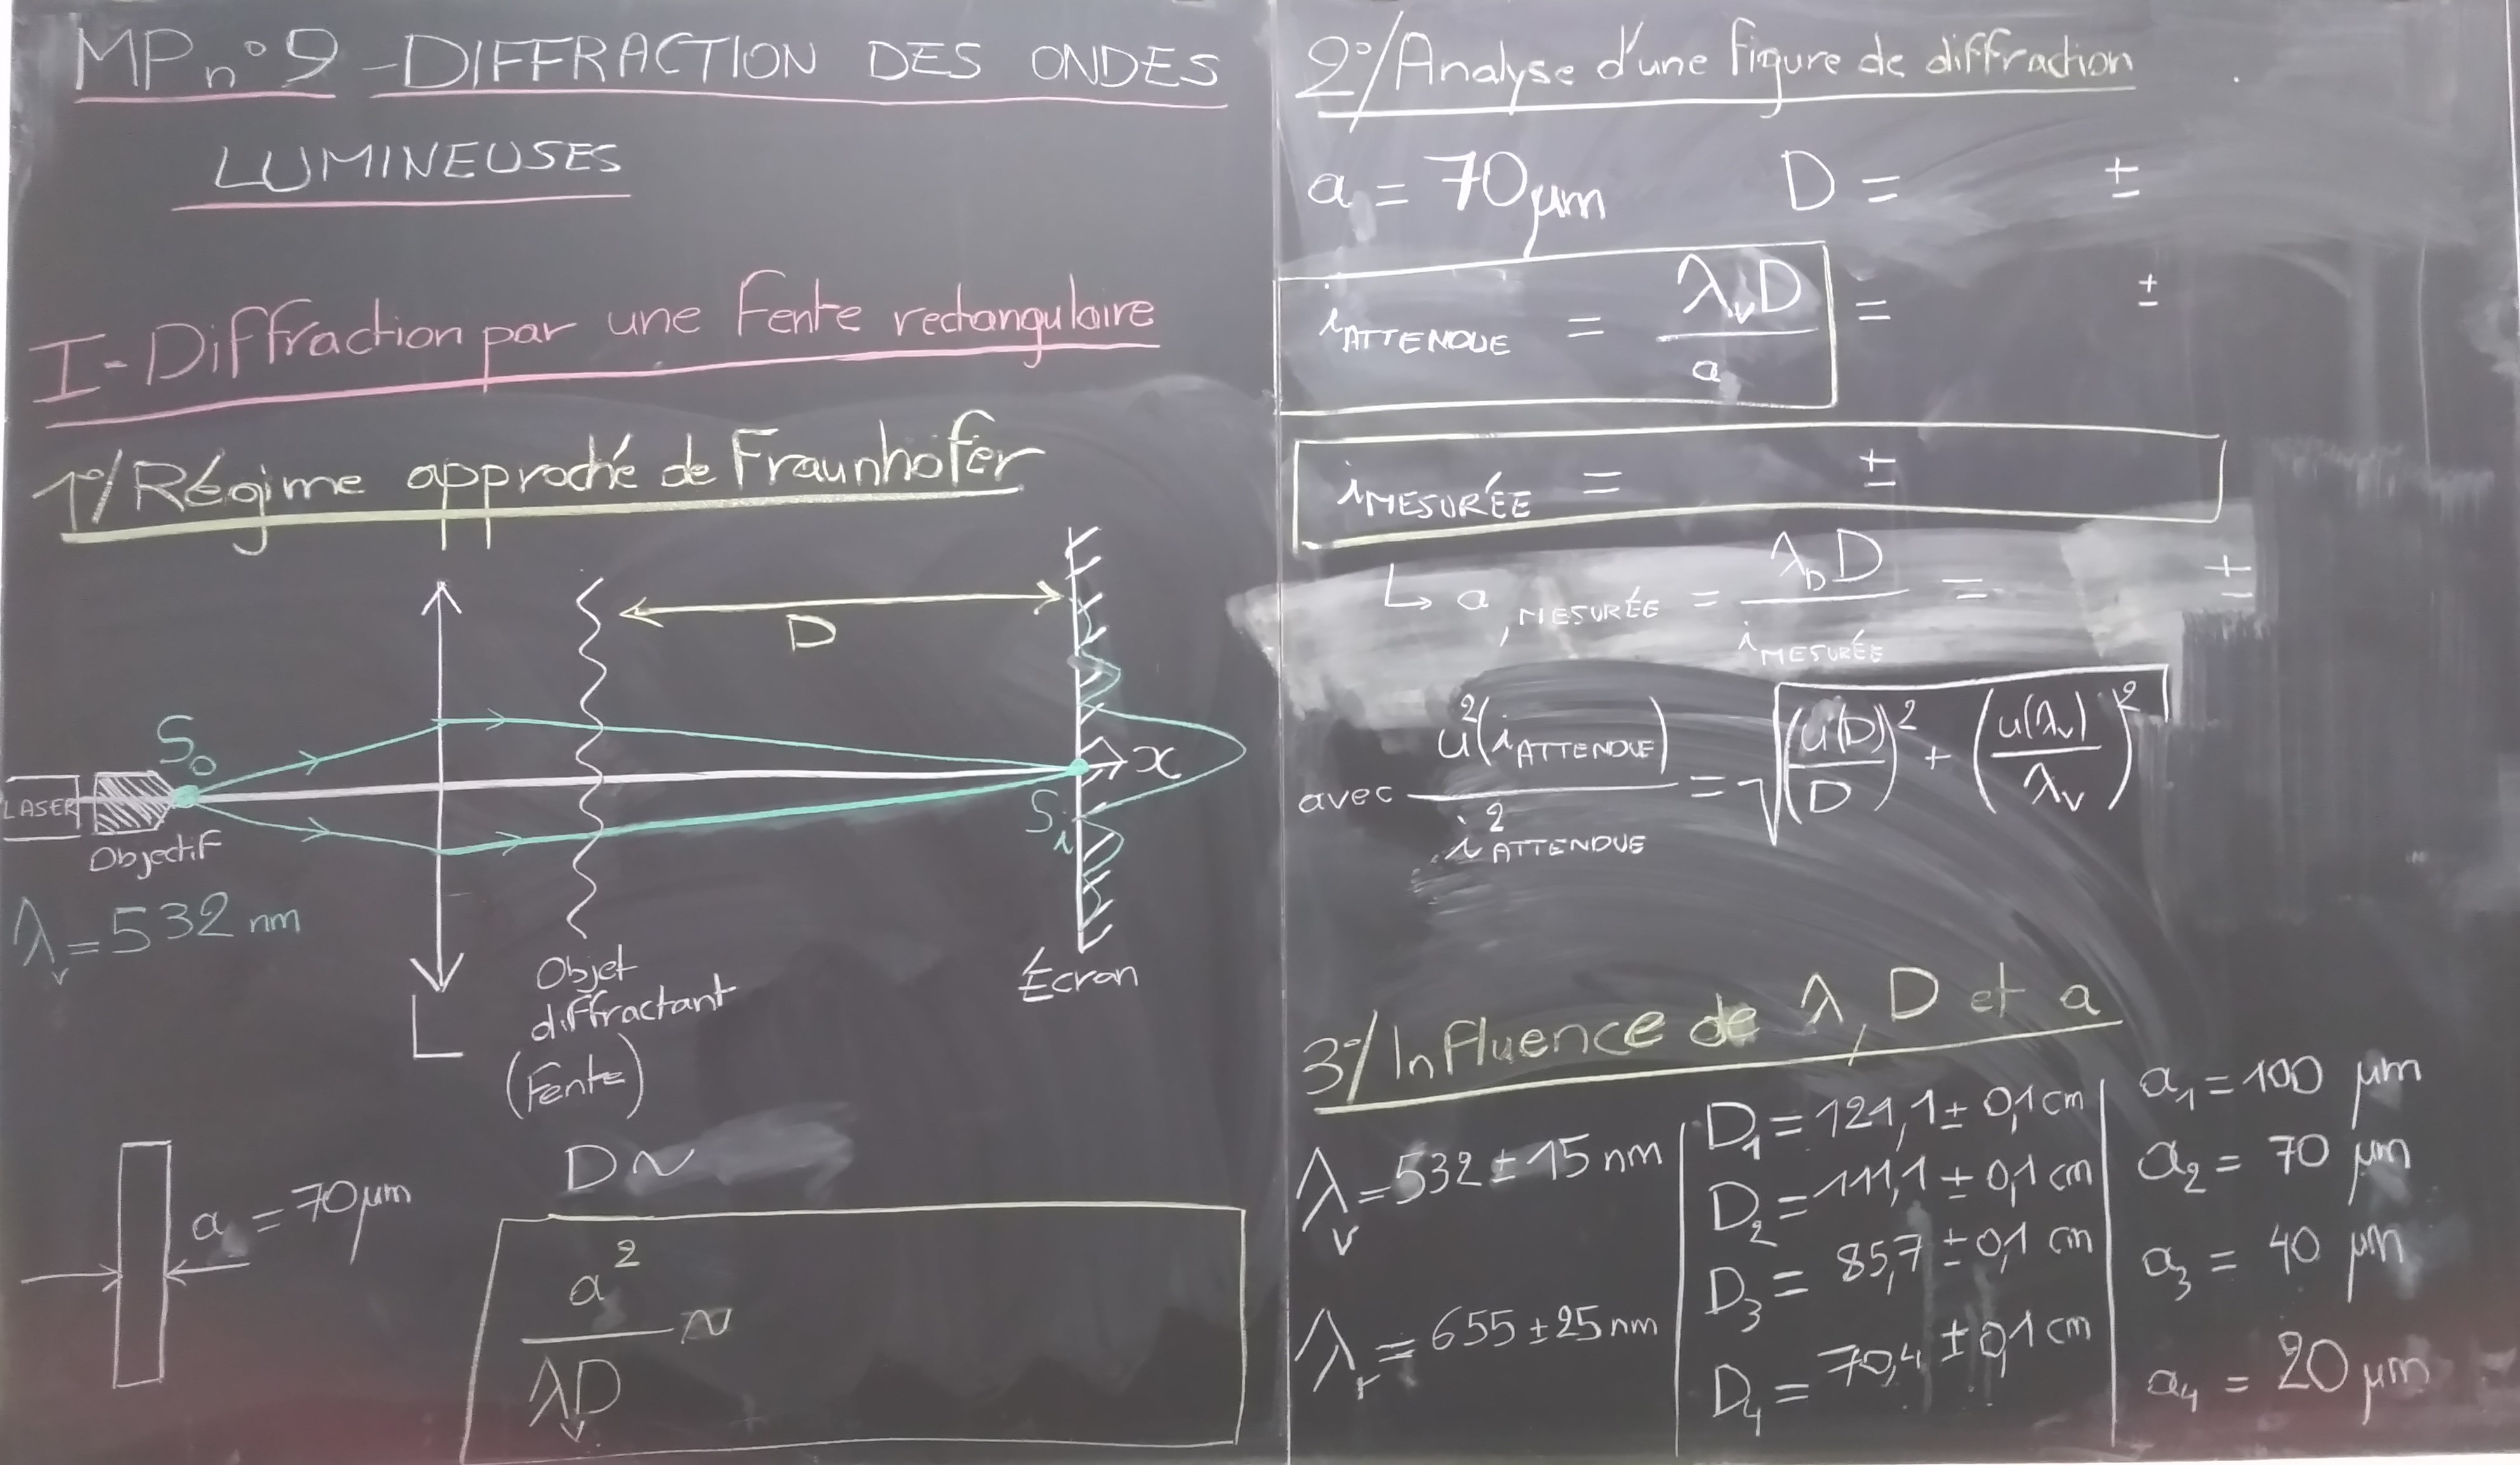
\includegraphics[width=18cm]{T1}}
\end{figure}
\begin{figure}[h]
	\centerline{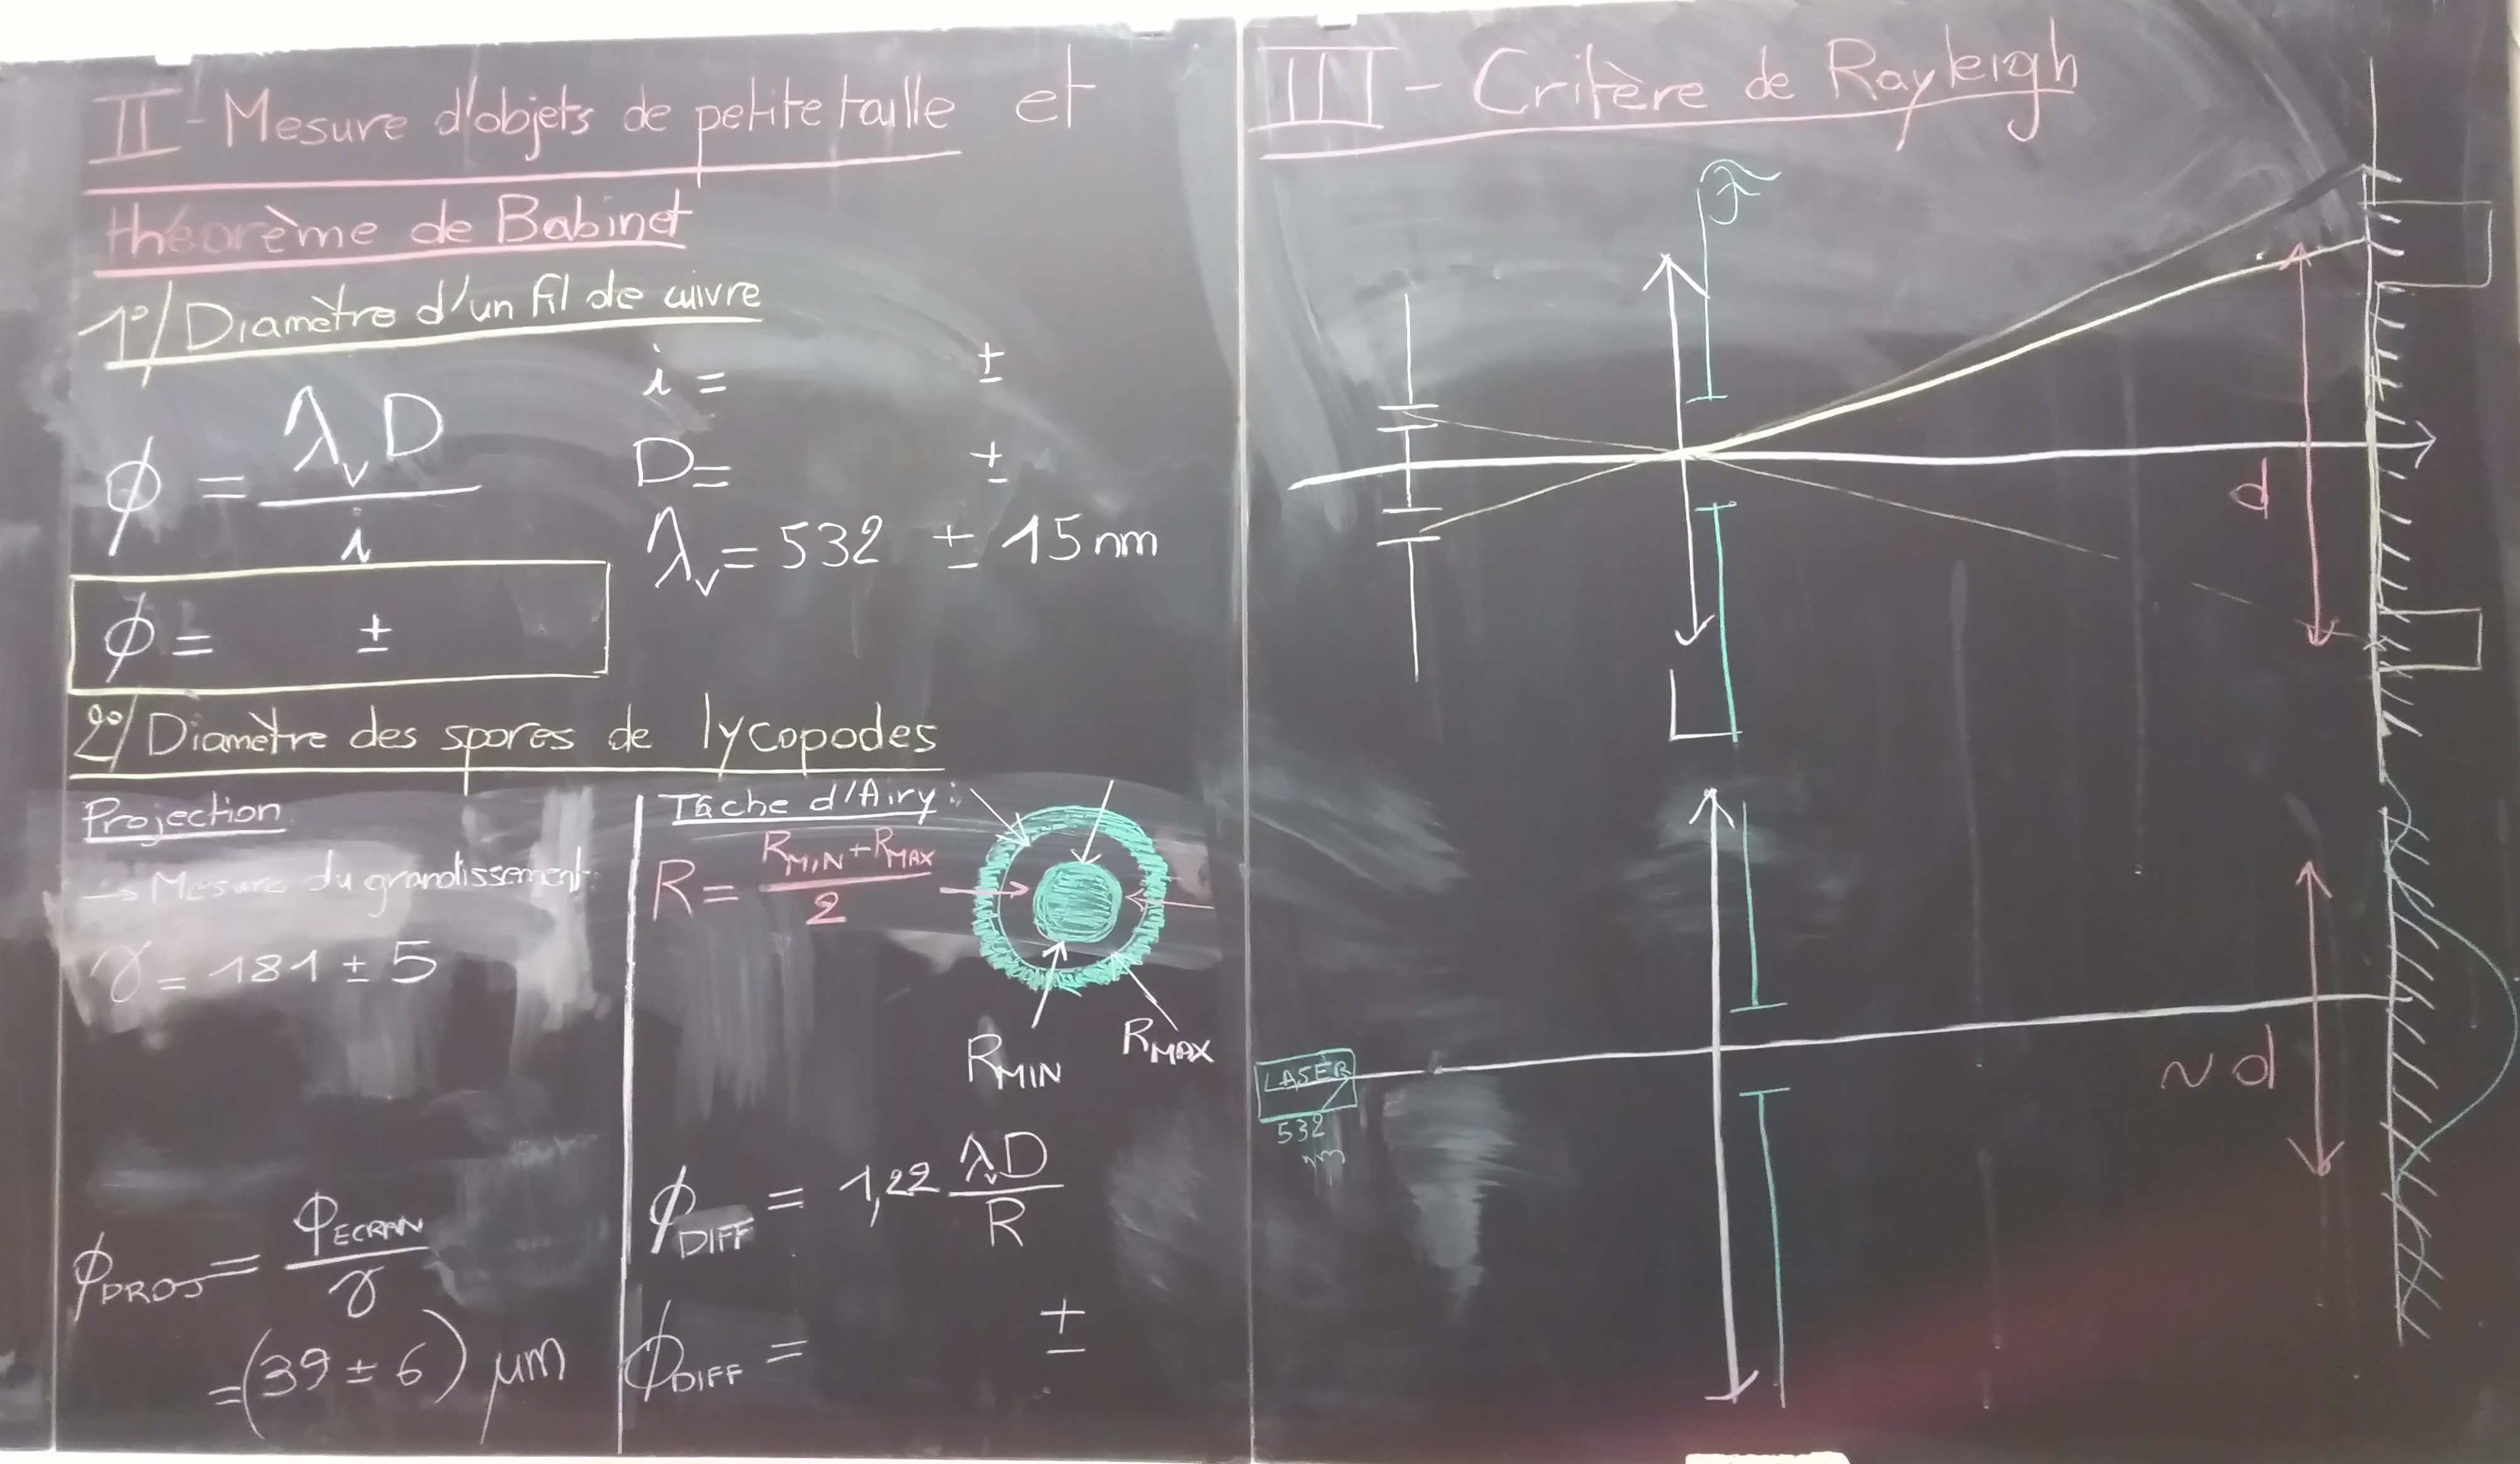
\includegraphics[width=18cm]{T2}}
\end{figure}

\subsection{Régime approché de Fraunhoffer}
La tache de diffraction se forme autour de l'image de la fente, donc si on translate la fente on translate de même la figure de diffraction.\\
Mesure de D, on montre que $\frac{a^2}{\lambda_0 D}\ll 1$ et que l'on est donc bien dans les conditions de Fraunhoffer approchée.

\subsection{Analyse d'une figure de diffraction}
On déduit des longueurs caractéristiques du problème la valeur de l'interfrange attendue en considérant $a=70\mu m$ et ayant mesuré $D= 123.0 +-0.1 cm$
\begin{eqnarray}
i_{attendu} = \frac{\lambda_0 D }{a} = 0.9 +- 0.1\;cm
\end{eqnarray}
Ici l'incertitude sur l'interfrange est surtout due à l'incertitude sur la longueur d'onde du laser $\lambda_0$.\\
On mesure ensuite $i$ en prenant la longueur séparant les extinctions successives, on rentre dans un tableau $l(n)$ où $n$ est le numéro de la énième extinction, et $l(n)$ la distance séparant la première extinction de la $n^{ieme}$, et on le trace. On obtient ainsi une droite $l=i_{mesure} n$ et on en déduit
\begin{eqnarray}
i_{mesuré} = 10.8 +- 4 mm \Rightarrow i_{mesuré} = 1.1 +- 1 cm
\end{eqnarray}  
On en déduit ainsi une mesure de a
\begin{eqnarray}
a_{mesure} = \frac{\lambda_0 D}{i_{mesure}} = 59 +- 6 \mu m
\end{eqnarray}
$\Rightarrow $ Pas en accord avec la valeur de a donnée par le constructeur .. sans doute dû à une mauvaise mesure de $i$ due à un pointage imprécis des extinctions.
\paragraph{FAUX :} l'erreur est fondamentale ici, dans cette configuration la théorie ne tient pas car l'objet n'est pas éclairée par une onde plane, et il est très compliqué de définir D ici...\\
$\Rightarrow$ Il faut donc utiliser 2 lentilles et alors $D\rightarrow f_i$ ou bien éclairer directement l'objet diffractant avec les faisceau laser qui est une succession d'ondes presque planes, de plus dans ce cas on a un maximum de lumière qui est transmise si on utilise une fente.

\subsection{Influence de $\lambda$, D et a}
On garde le même montage ici.\\
On constate que lorsque la largeur des taches augmente, due au passage d'un laser vert à un laser rouge, la courbe $l(n)$ devient plus imprécise. C'est normal étant donné que les extinctions sont donc plus difficile à pointer. La courbe d'étalonnage représentant $i(a)$ sera donc réalisée avec le laser vert.

\section{Mesure d'objets de petite taille et théorème de Babinet}
On peut mesurer le diamètre d'un objet diffractant comme étant 
\begin{eqnarray}
\phi = \frac{\lambda_0 D}{i}
\end{eqnarray}
on peut notamment utiliser la courbe d'étalonnage réalisée précédemment avec différentes valeur de a (4) pour trouver la taille caractéristique de l'objet mesuré. 

\subsection{Diamètre d'un fil de cuivre}
On mesure ici le diamètre d'un fil de cuivra ayant une épaisseur tabulée de $70\mu m$ (ce qui correspond à la largeur d'une des fentes utilisée précédemment $\rightarrow$ on pourrait donc faire une comparaison directe des taches de diffraction (dans la direction x seulement, puisque c'est l'unique direction pour laquelle les largeurs caractéristiques sont les mêmes)). \\
Ici on mesure 
\begin{eqnarray}
i = 8.4 +- 0.1 mm\; \rightarrow \phi = \frac{\lambda_0 D}{i} = 77 +-3 \mu m
\end{eqnarray}
(où on a à nouveau négligé l'incertitude sur $D$). Cela ne correspond pas avec la valeur tabulé.

\subsection{Diamètre des spores de lycopodes}
Le th de Babinet nous prédit l'apparition d'une tache d'Airy puisque l'objet diffractant est circulaire. On constate qu'il y a une seule figure de diffraction malgré la multitude de spores éclairés, c'est parce que une translation de l'objet diffractant n'impacte pas la figure de diffraction à l'infini (ici dans le plan focal image de la lentille convergente).\\
On peut comparer le résultat obtenu en utilisant la diffraction à ceux obtenus en utilisant la projection de l'image des spores par un objectif de microscope sur un écran, après avoir mesuré le grandissement de ce dispositif grâce à une mire.

\section{Critère de Reyleigh}


\section{Questions}
\subsubsection{Pour le critère de Reyleigh :}
Q'entendez vous par largeur des bi-fentes ?\\

La figure de diffraction se forme autour de quel point ? Si c'est autour de l'image du centre de l'objet (point à mi chemin entre les deux fentes) elle se forme donc autour d'un point sombre ?\\

Dans le cadre du montage lié au critère de Reyleigh, où faut il placer le condenseur et l'objet afin d'observer une figure nette ?\\
il faut faire l'image du filament par le condenseur sur la fente afin d'avoir un max de lumière.

\subsubsection{Pour le fil de cuivre :}
Différence entre diamètre, épaisseur, largeur... qu'est ce que vous mesurez ?\\
Un fil est un objet tridimensionnel, tandis qu'une fente est un objet bidimensionnel, l'étendue spatiale de l'objet n'impacte elle pas la figure de diffraction ?
\subsubsection{Pour la partie 1 :}
Concernant la figure $i(a)$ : que représente l'ordonnée à l'origine de la droite du modèle affine ?\\ 

Pourquoi avoir écarter les erreurs systématiques ? Tandis que cela aurait du mettre en valeur le non accord entre la théorie invoquée et les résultats observés. \\

\section{Remarques}
Montage de diffraction : l'objet diffractant doit être éclaire par une onde plane !\\
Par conséquent les erreurs systématiques sont dues au fait au'on utilise une seule lentille et non 2 : donc la distance D n'est pas bien définie au niveau théorique, car on ne sait pas où placer l'objet entre la lentille et l'écran placé de telle sorte à ce que l'cran soit le conjugué du point source (focale de l'objectif de microscope) par la lentille.\\
Concernant le laser : processus interne très complexe relevant de l'optique non linéaire, et permettant d'émettre à une longueur d'onde EXTRÊMEMENT précise. L'incertitude constructeur concerne donc la garantie sur la valeur de la longueur d'onde du laser acheté en particulier. Il faut donc faire une mesure de $\lambda_0$ pour avoir une incertitude réaliste sur cette longueur d'onde, qui est très faible.\\
Possibilité donc de faire une petite manip de spectro en intro pour acractériser le laser.\\
Attention à la forme donc sur ce genre de montage.\\
On ne mesure pas l'interfrange ici, notamment sur $l(n)$, mais une distance entre une origine arbitraire et les extinctions. Le zéro doit être pris au centre, là où $sinc(0) = 1$, de plus on fait une régression affine car on mesure une distance : il n'y a pas d'origine fixe, on fixe l'origine de la règle de manière complètement arbitraire.\\
remarque : ici il est facile de prendre une mesure en directe et de l'ajouter à la courbe puisque les éléments optiques sont fixés sur le banc.\\
Devant une figure explicitement fausse : ilne faut pas en appeler à sa maladresse ou à des erreurs de pointage... il faut conclure que la manip est fausse et ne s'inscrit pas dans le cadre du modèle développé.\\
On a que 30 minutes : trop long. En plus ici les manip sont sensiblement les mêmes.\\
Enlever la manip avec le fil car objet étendu et donc compliqué à traiter analytiquement.\\
Pour ce qui est de faire varier $\lambda_0$, $D$ et $a$ : faire seulement 2 valeurs de chaque paramètre par manque de temps, et mesurer $i$ en prenant les plus d'extinctions possibles.\\
Pour les lycopodes : plutôt montrer la mesure du microscope qui est de nature différente, ou bien enlever cette manip si pas le temps.\\
Pour Rayleigh : difficile de faire quantitatif. \\
Possibilité de faire manip du filtrage d'Abbes, mais dans ce cas virer la partie 1.\\
Donc manip 2 + lycopodes + Reyleigh ou Abbes.\\

Faire très attention à tout le vocabulaire pour ce qi est des distances, épaisseur, largeur, longueur, diamètre, écart, etc... Attention à l'emploi du mot interfrange qui n'est pas adapté à la diffraction mais aux interférences. dire distance entre les extinctions/annulation de l'éclairement.\\
Attention au vocabulaire "tabulé" mal employé ici : il faut dire "donnée par le constructeur".



\end{document}
